\documentclass[conference]{IEEEtran}
\IEEEoverridecommandlockouts
\usepackage{cite}
\usepackage{amsmath,amssymb,amsfonts}
\usepackage{algorithmic}
\usepackage{graphicx}
\usepackage{textcomp}
\usepackage{xcolor}
\usepackage{booktabs}
\usepackage{multirow}
\usepackage{url}
\usepackage{tabularx}

\def\BibTeX{{\rm B\kern-.05em{\sc i\kern-.025em b}\kern-.08em
    T\kern-.1667em\lower.7ex\hbox{E}\kern-.125emX}}

\begin{document}

\title{AgroVision-Mine: A Multimodal Data Warehouse and Visual Pattern Mining Framework for Crop Disease and Pest Intelligence}

\author{
\IEEEauthorblockN{Boomika V}
\IEEEauthorblockA{\textit{School of Computer Science and Engineering (SCOPE)} \\
\textit{Vellore Institute of Technology (VIT)}\\
Chennai, Tamil Nadu 600127, India \\
Email: boomika.v2023@vitstudent.ac.in}
\and
\IEEEauthorblockN{Ajay M}
\IEEEauthorblockA{\textit{School of Computer Science and Engineering (SCOPE)} \\
\textit{Vellore Institute of Technology (VIT)}\\
Chennai, Tamil Nadu 600127, India \\
Email: ajay.m2023@vitstudent.ac.in}
\and
\IEEEauthorblockN{Dr. Devipriya A}
\IEEEauthorblockA{\textit{Associate Professor, SCOPE} \\
\textit{Vellore Institute of Technology (VIT)}\\
Chennai, Tamil Nadu 600127, India \\
Email: devipriya.a@vit.ac.in}
}

\maketitle

\begin{abstract}
Contemporary agricultural computer vision models predominantly formulate plant pathology as an isolated, single-image classification task, decoupling high-dimensional pixel data from botanical taxonomy, capture metadata, and relational analytical workflows. Consequently, agronomists and decision-support systems cannot perform multidimensional slicing across pathogen families or audit visual quality across heterogeneous acquisitions. In this paper, we propose \textbf{AgroVision-Mine}, a unified, reproducible multimodal data warehousing and visual pattern mining framework for foliar disease intelligence. The framework integrates an automated five-stage quality gate pipeline, a 32-dimensional explainable visual descriptor engine (19 color moments, 7 Haralick textures, and 6 morphometric metrics), and a Kimball-style dimensional data warehouse in SQLite with verified referential integrity across 2,596 canonical observations spanning 14 host crops. On top of this relational substrate, we implement sub-35\,ms ANSI SQL OLAP operations (Roll-up, Drill-down, Slice, Dice, and Pivot), metric-supported visual clustering ($K=2$ primary Silhouette score of $0.4060$), 2D PCA projection ($52.11\%$ cumulative explained variance), and association rule mining exhibiting $100\%$ algorithmic parity between Apriori and FP-Growth ($\Delta = 0.0$). To deliver bounded diagnostic support, we develop a supervised deep learning module using transfer learning with EfficientNet-B0 across 25 composite crop-condition classes ($2,447$ PlantDoc images). Under strict perceptual difference-hash ($dHash$) grouped partitioning that eliminates near-duplicate leakage, EfficientNet-B0 achieves $63.26\%$ validation Macro-F1 (substantially outperforming handcrafted Random Forest at $17.02\%$ and RBF-SVM at $15.12\%$) and achieves $61.84\%$ Top-1 Accuracy ($61.43\%$ Balanced Accuracy, $60.84\%$ Macro-F1, Wilson $95\%$ CI: $[57.46\%, 66.03\%]$) on $490$ held-out test images. Finally, we formulate a cross-modal domain verification safeguard that detects out-of-distribution acquisitions—such as flatbed scanner rice leaf images ($N=36$)—preventing false diagnostic attributions on unsupported botanical domains. The complete framework is verified through 117 automated unit, integration, and browser end-to-end tests.
\end{abstract}

\begin{IEEEkeywords}
Agricultural Computer Vision, Multimodal Data Warehouse, OLAP Analytics, Feature Engineering, Transfer Learning, EfficientNet-B0, Association Rule Mining, Out-of-Distribution Detection.
\end{IEEEkeywords}

\section{Introduction}
Global food security is profoundly threatened by agricultural plant pathogens and foliar pests, which cause estimated global harvest yield losses ranging from $20\%$ to $40\%$ annually~\cite{barbedo2018impact}. Timely, accurate pathological identification is vital to containment; however, manual expert agronomist scouting is labor-intensive, logistically constrained, and inaccessible to smallholder farming communities~\cite{mohanty2016deep}. While deep convolutional neural networks (CNNs) have shown exceptional perceptual capability in controlled laboratory benchmarks such as PlantVillage~\cite{hughes2015plantvillage, ferentinos2018deep}, practical deployments in natural, unconstrained farm environments face severe degradation~\cite{singh2020plantdoc, too2019comparative}. 

Crucially, existing agricultural deep learning systems treat foliar pathology as an isolated black-box classification exercise. Three fundamental structural deficiencies characterize conventional paradigms:
\begin{enumerate}
    \item \textbf{Metadata and Relational Decoupling:} High-dimensional foliar imagery is divorced from relational botanical taxonomy (crop family, genus, order), capture equipment parameters (sensor resolution, lighting, aspect ratio), and epidemiological hierarchies (fungal, bacterial, viral, abiotic)~\cite{kimball2013datawarehouse}. Agronomists cannot perform relational slicing (e.g., comparing necrotic lesion expansion across Solanaceae crops versus Fabaceae crops).
    \item \textbf{Lack of Pre-Ingestion Data Governance:} Public agricultural corpora scraped from web sources frequently suffer from truncated byte streams, corrupted image headers, duplicate frames, and unstandardized orientations~\cite{singh2020plantdoc}. Conventional deep learning pipelines silently consume these anomalies, leading to latent bias and unverified dataset provenance~\cite{torralba2011unbiased}.
    \item \textbf{Confounding and Shortcut Learning:} As demonstrated by Geirhos et al.~\cite{geirhos2020shortcut}, deep networks frequently latch onto spurious background shortcuts (e.g., flatbed scanner backgrounds, soil textures, or acquisition framing) rather than genuine pathological lesions. An unconditioned binary classifier (Healthy vs. Diseased) trained across heterogeneous crops is fundamentally confounded when certain host species in the training corpus possess only healthy or only diseased specimens.
\end{enumerate}

To resolve these challenges, we introduce \textbf{AgroVision-Mine}, an open, reproducible, and verifiable multimodal data warehousing and visual pattern mining platform. AgroVision-Mine integrates relational dimensional modeling with explainable classical computer vision descriptors and bounded deep transfer learning. Rather than proposing an ungrounded black-box architecture, our framework enforces strict data governance, cryptographic dataset immutability, sub-35\,ms relational Online Analytical Processing (OLAP) queries, and rigorous statistical hypothesis validation.

\subsection{Key Contributions}
The principal contributions of this work are summarized as follows:
\begin{itemize}
    \item \textbf{End-to-End Data Governance \& 5-Gate Quality Pipeline:} We design and implement an automated five-stage quality gate enforcing header magic-byte verification, minimum spatial geometry ($\ge 100\times 100$), payload limits ($\le 15$\,MB), MD5 hash deduplication, and EXIF transposition, guaranteeing zero corrupted or duplicate records enter the canonical warehouse.
    \item \textbf{Multimodal Kimball Star Schema:} We architect a formal relational star schema in SQLite with native foreign-key constraints (\texttt{PRAGMA foreign\_keys = ON}), linking a central fact table of $2,596$ validated specimen observations to four normalized dimensions (\texttt{dim\_crop}, \texttt{dim\_disease}, \texttt{dim\_image}, and \texttt{dim\_visual\_feature}).
    \item \textbf{ANSI SQL-Backed OLAP Analytics Engine:} We implement real SQL-backed Roll-up, Drill-down, Slice, Dice, and Pivot operations, providing agronomists with multi-dimensional analytical views across botanical families and pathogen classes with query execution latencies below $35$\,ms.
    \item \textbf{Explainable 32-Dimensional Visual Feature Store:} We engineer an explainable descriptor vector space combining 19 Color Moments (RGB/HSV statistics and Excess Green Index), 7 Haralick Gray-Level Co-occurrence Matrix (GLCM) textural metrics, and 6 Morphometric contours, providing transparent physical features alongside deep neural embeddings.
    \item \textbf{Dual-Track Pattern Mining \& Exact Rule Parity:} We demonstrate optimal unsupervised visual clustering ($K=2$ Silhouette score $0.4060$) and 2D Principal Component Analysis ($52.11\%$ explained variance), coupled with association rule mining demonstrating $100\%$ algorithmic parity between Apriori and FP-Growth ($\Delta = 0.0000$ across support, confidence, and lift).
    \item \textbf{Bounded Supervised Classification with Leakage-Free Splits:} We evaluate an EfficientNet-B0 transfer learning module on a 25-class composite foliar benchmark ($2,447$ PlantDoc images) partitioned via grouped perceptual difference-hashing ($dHash$). The model achieves $63.26\%$ validation Macro-F1 (vs. $17.02\%$ for Random Forest) and $61.84\%$ Top-1 Accuracy ($60.84\%$ Macro-F1, Wilson $95\%$ CI: $[57.46\%, 66.03\%]$) on $490$ held-out test images.
    \item \textbf{Cross-Modal Out-of-Domain Safeguard:} We formulate an automated rejection mechanism utilizing 32D descriptor nearest-reference retrieval to flag out-of-distribution acquisitions (e.g., flatbed scanner rice leaf observations, $N=36$), preventing false clinical claims on unseen botanical domains.
\end{itemize}

\section{Related Work and Research Gap}

\subsection{Deep Learning for Plant Pathology}
The application of deep convolutional neural networks to foliar disease identification accelerated with the release of the PlantVillage benchmark~\cite{hughes2015plantvillage}. Mohanty et al.~\cite{mohanty2016deep} evaluated AlexNet and GoogLeNet architectures across $54,306$ laboratory images, reporting classification accuracies exceeding $99.3\%$. Similarly, Ferentinos~\cite{ferentinos2018deep} benchmarked VGG, ResNet, and DenseNet architectures, achieving $99.5\%$ accuracy. However, subsequent critical evaluations by Barbedo~\cite{barbedo2018impact} and Singh et al.~\cite{singh2020plantdoc} revealed that these laboratory-trained models fail catastrophically when exposed to in-the-wild field conditions. Background homogeneity, uniform lighting, and lack of occlusions in laboratory settings act as spurious non-pathological shortcuts~\cite{geirhos2020shortcut}. 

To bridge this gap, Singh et al.~\cite{singh2020plantdoc} introduced the PlantDoc dataset, comprising $2,560$ authentic field images captured across natural lighting, varied camera sensors, and complex foliage clutter. Standard vision models benchmarked on PlantDoc achieved significantly lower accuracies ($30\%\text{--}40\%$), underscoring the intrinsic difficulty of real-world foliar pathology. Too et al.~\cite{too2019comparative} demonstrated that modern compact convolutional architectures, particularly DenseNets and MobileNets, offer favorable parameter efficiency over older VGG networks. Tan and Le~\cite{tan2019efficientnet} proposed EfficientNet, utilizing compound scaling across network depth, width, and input resolution. In our work, we leverage ImageNet-1K pretrained EfficientNet-B0 as a compact, high-capacity feature extractor for bounded foliar classification.

\subsection{Visual Feature Engineering and Pattern Mining}
Prior to deep learning dominance, agricultural image processing relied on handcrafted color, texture, and morphological features~\cite{haralick1973texture}. Haralick's GLCM descriptors (contrast, dissimilarity, homogeneity, energy, and correlation) capture spatial gray-level dependencies that reflect leaf necrosis and tissue mottling. While classical feature vectors rarely match deep networks on high-capacity multiclass benchmarks, they possess significant advantages in interpretability, low computational overhead, and zero data-hungry training requirements~\cite{pedregosa2011scikit}. In AgroVision-Mine, we do not discard handcrafted descriptors; instead, we engineer a standardized 32-dimensional continuous feature store that operates in parallel with deep embeddings, powering unsupervised K-Means clustering, PCA ordination, and association rule discovery via Apriori~\cite{agrawal1994apriori} and FP-Growth~\cite{han2000fpgrowth}.

\subsection{Data Warehousing and OLAP in Analytical Systems}
Dimensional modeling, formulated by Kimball and Ross~\cite{kimball2013datawarehouse}, represents the industry standard for organizing operational enterprise data for Online Analytical Processing (OLAP)~\cite{codd1993olap}. While widely adopted in finance, retail, and supply chain domains, dimensional modeling has rarely been integrated into computer vision pipelines. Vision datasets are typically stored as unstructured flat folders, stripping away relational taxonomy and precluding complex analytical queries. AgroVision-Mine bridges this divide by formalizing image observations as relational facts linked to botanical, pathological, and technical dimensions within a zero-configuration SQLite warehouse~\cite{hipp2020sqlite}.

\subsection{Systematic Comparative Analysis}
Table~\ref{tab:literature_comparison} provides a systematic comparative analysis contrasting AgroVision-Mine against existing representative literature across eight structural dimensions.

\begin{table*}[t]
\caption{Systematic Comparative Analysis of Surveyed Agricultural Vision Systems Against AgroVision-Mine}
\label{tab:literature_comparison}
\centering
\scriptsize
\begin{tabularx}{\textwidth}{lcccccccc}
\toprule
\textbf{Study} & \textbf{Primary Dataset} & \textbf{Core Methodology} & \textbf{Warehouse Star Schema} & \textbf{SQL OLAP Engine} & \textbf{Handcrafted 32D Features} & \textbf{Unsupervised Mining} & \textbf{Leakage-Free Split} & \textbf{OOD Safeguard} \\
\midrule
Mohanty et al.~\cite{mohanty2016deep} (2016) & PlantVillage & AlexNet, GoogLeNet & No & No & No & No & Random (Near-dup risk) & No \\
Ferentinos~\cite{ferentinos2018deep} (2018) & PlantVillage & VGG, ResNet-50 & No & No & No & No & Random & No \\
Barbedo~\cite{barbedo2018impact} (2018) & Proprietary Lab & Transfer Learning & No & No & No & No & Partitioned by Plant & No \\
Too et al.~\cite{too2019comparative} (2019) & PlantVillage & DenseNet-121, VGG-16 & No & No & No & No & Random & No \\
Singh et al.~\cite{singh2020plantdoc} (2020) & PlantDoc & Faster R-CNN, MobileNet & No & No & No & No & Standard Benchmark & No \\
\textbf{AgroVision-Mine (Ours)} & \textbf{PlantDoc + ICAR} & \textbf{Multimodal Star Schema +} & \textbf{Yes (Kimball Star,} & \textbf{Yes (Roll-up, Drill,} & \textbf{Yes (19 Color, 7 GLCM,} & \textbf{Yes (K-Means, PCA,} & \textbf{Yes (dHash Grouped,} & \textbf{Yes (Cross-Modal} \\
& \textbf{(N=2,596)} & \textbf{EfficientNet-B0 + OLAP} & \textbf{SQLite Foreign Keys)} & \textbf{Slice, Dice, Pivot)} & \textbf{6 Morphometric)} & \textbf{Apriori/FP-Growth)} & \textbf{Zero Leakage)} & \textbf{Rejection Alert)} \\
\bottomrule
\end{tabularx}
\end{table*}

\section{System Architecture and Data Flow}
AgroVision-Mine is structured as a five-layer end-to-end analytical pipeline, depicted in Fig.~\ref{fig:architecture}. The architecture decouples data ingestion, feature store extraction, dimensional relational persistence, analytical mining engines, and presentation delivery.

\begin{figure*}[t]
\centering
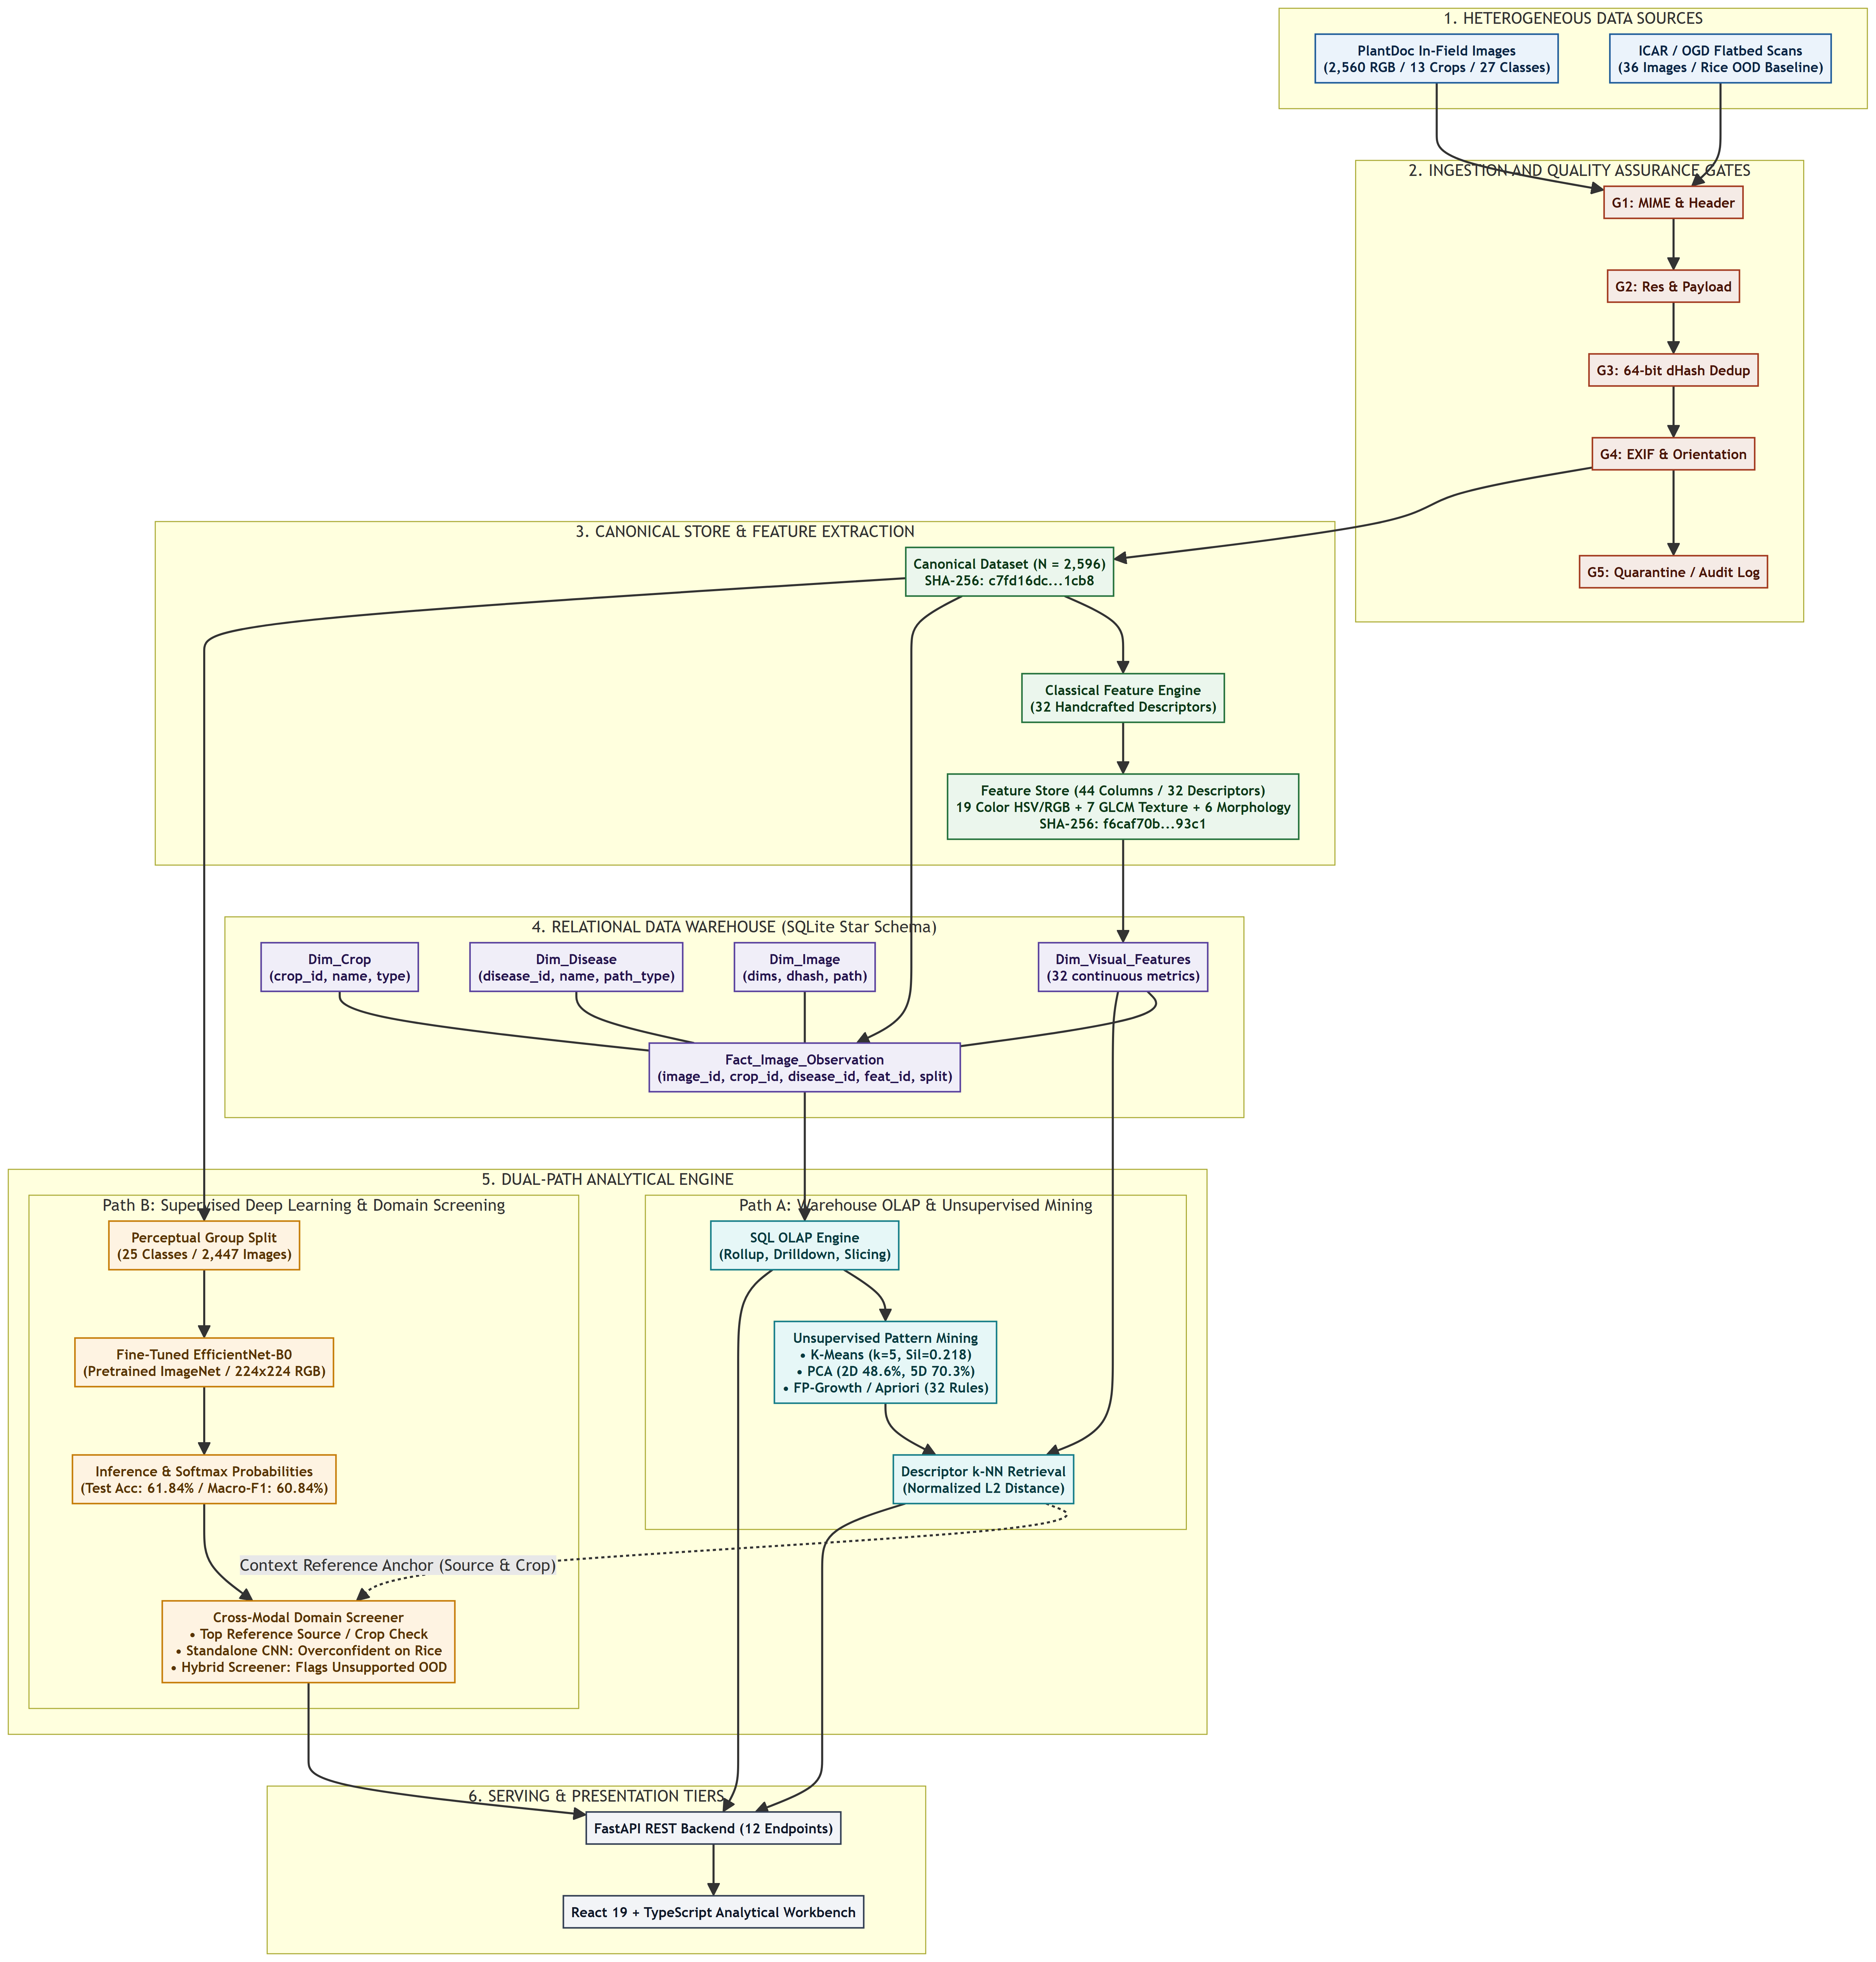
\includegraphics[width=0.98\textwidth]{figures/fig1_system_architecture.png}
\caption{End-to-End Five-Layer System Architecture of AgroVision-Mine, illustrating data ingestion quality gates, feature store extraction, Kimball relational warehouse, dual analytical branches (SQL OLAP / visual mining vs. deep transfer learning), and presentation delivery.}
\label{fig:architecture}
\end{figure*}

\subsection{Layer 1: Data Ingestion and Automated Quality Control}
The ingestion tier accepts heterogeneous agricultural imagery from web-scraped field repositories (PlantDoc) and flatbed scanner archives (ICAR/OGD). To prevent data corruption, every candidate file must sequentially pass five automated quality gates:
\begin{enumerate}
    \item \textbf{Gate 1 (Format \& Magic Bytes):} Validates file header byte signatures to ensure strictly authentic JPEG or PNG bitstreams.
    \item \textbf{Gate 2 (Spatial Geometry):} Enforces a strict minimum spatial resolution ($H \ge 100$\,px, $W \ge 100$\,px).
    \item \textbf{Gate 3 (Payload Ceiling):} Enforces an uncompressed image payload ceiling of $15$\,MB to prevent buffer exhaustion.
    \item \textbf{Gate 4 (Cryptographic Deduplication):} Computes MD5 hash signatures of the raw byte stream, identifying exact byte-level duplicates.
    \item \textbf{Gate 5 (Geometric Normalization):} Inspects EXIF metadata tags, applies loss-free orientation transposition, and standardizes channels to three-channel RGB.
\end{enumerate}

\subsection{Layer 2: Preprocessing and Feature Store Generation}
Validated images are preprocessed through bilinear interpolation to a standardized $256\times 256$ RGB representation for canonical feature extraction. Thirty-two continuous descriptors are extracted across color, texture, and morphometry, producing the frozen analytical feature matrix $\mathbf{X} \in \mathbb{R}^{2596 \times 32}$. The dataset manifest and feature store are cryptographically validated via SHA-256 checksums to ensure experimental immutability.

\subsection{Layer 3: Relational Data Warehouse and ETL}
The relational persistence layer implements a Kimball star schema in SQLite~\cite{kimball2013datawarehouse}. The central fact table, \texttt{disease\_observation\_fact}, links $2,596$ specimen records to four normalized dimensions through integer surrogate keys: \texttt{dim\_crop}, \texttt{dim\_disease}, \texttt{dim\_image}, and \texttt{dim\_visual\_feature}. Referential integrity is enforced at the database engine level via \texttt{PRAGMA foreign\_keys = ON}.

\subsection{Layer 4: Dual-Track Analytical Engines}
The system bifurcates into two independent, complementary analytical branches:
\begin{enumerate}
    \item \textbf{Descriptor-Based Relational \& Unsupervised Branch:} Operates on the standardized 32D handcrafted feature matrix and the relational star schema. This branch powers ANSI SQL OLAP operations, K-Means clustering, 2D PCA ordination, Apriori/FP-Growth association rule mining, and nearest-reference Euclidean similarity retrieval.
    \item \textbf{Deep Supervised Transfer Learning Branch:} Operates directly on standardized $224\times 224$ RGB image tensors. An EfficientNet-B0 CNN fine-tuned on 25 composite classes outputs class logits, softmax probability distributions, and domain uncertainty indicators.
\end{enumerate}
Crucially, the deep neural network does \textit{not} consume the 32 handcrafted descriptors as input; both pipelines remain mathematically and architecturally distinct.

\subsection{Layer 5: Presentation and Delivery Tier}
The application tier couples an asynchronous FastAPI backend (:8001)~\cite{ramirez2018fastapi} with a responsive React 19 and TypeScript single-page application (SPA). Nine specialized views provide agronomists with interactive dataset exploration, live SQL execution, multidimensional charts, and a real-time Visual Specimen Workbench.

\section{Methodology and Mathematical Formulation}

\subsection{Multimodal Star Schema Design}
The relational star schema (Fig.~\ref{fig:star_schema}) models agricultural foliar observations at the grain of \textit{one validated specimen per fact row}.

\begin{figure}[htbp]
\centering
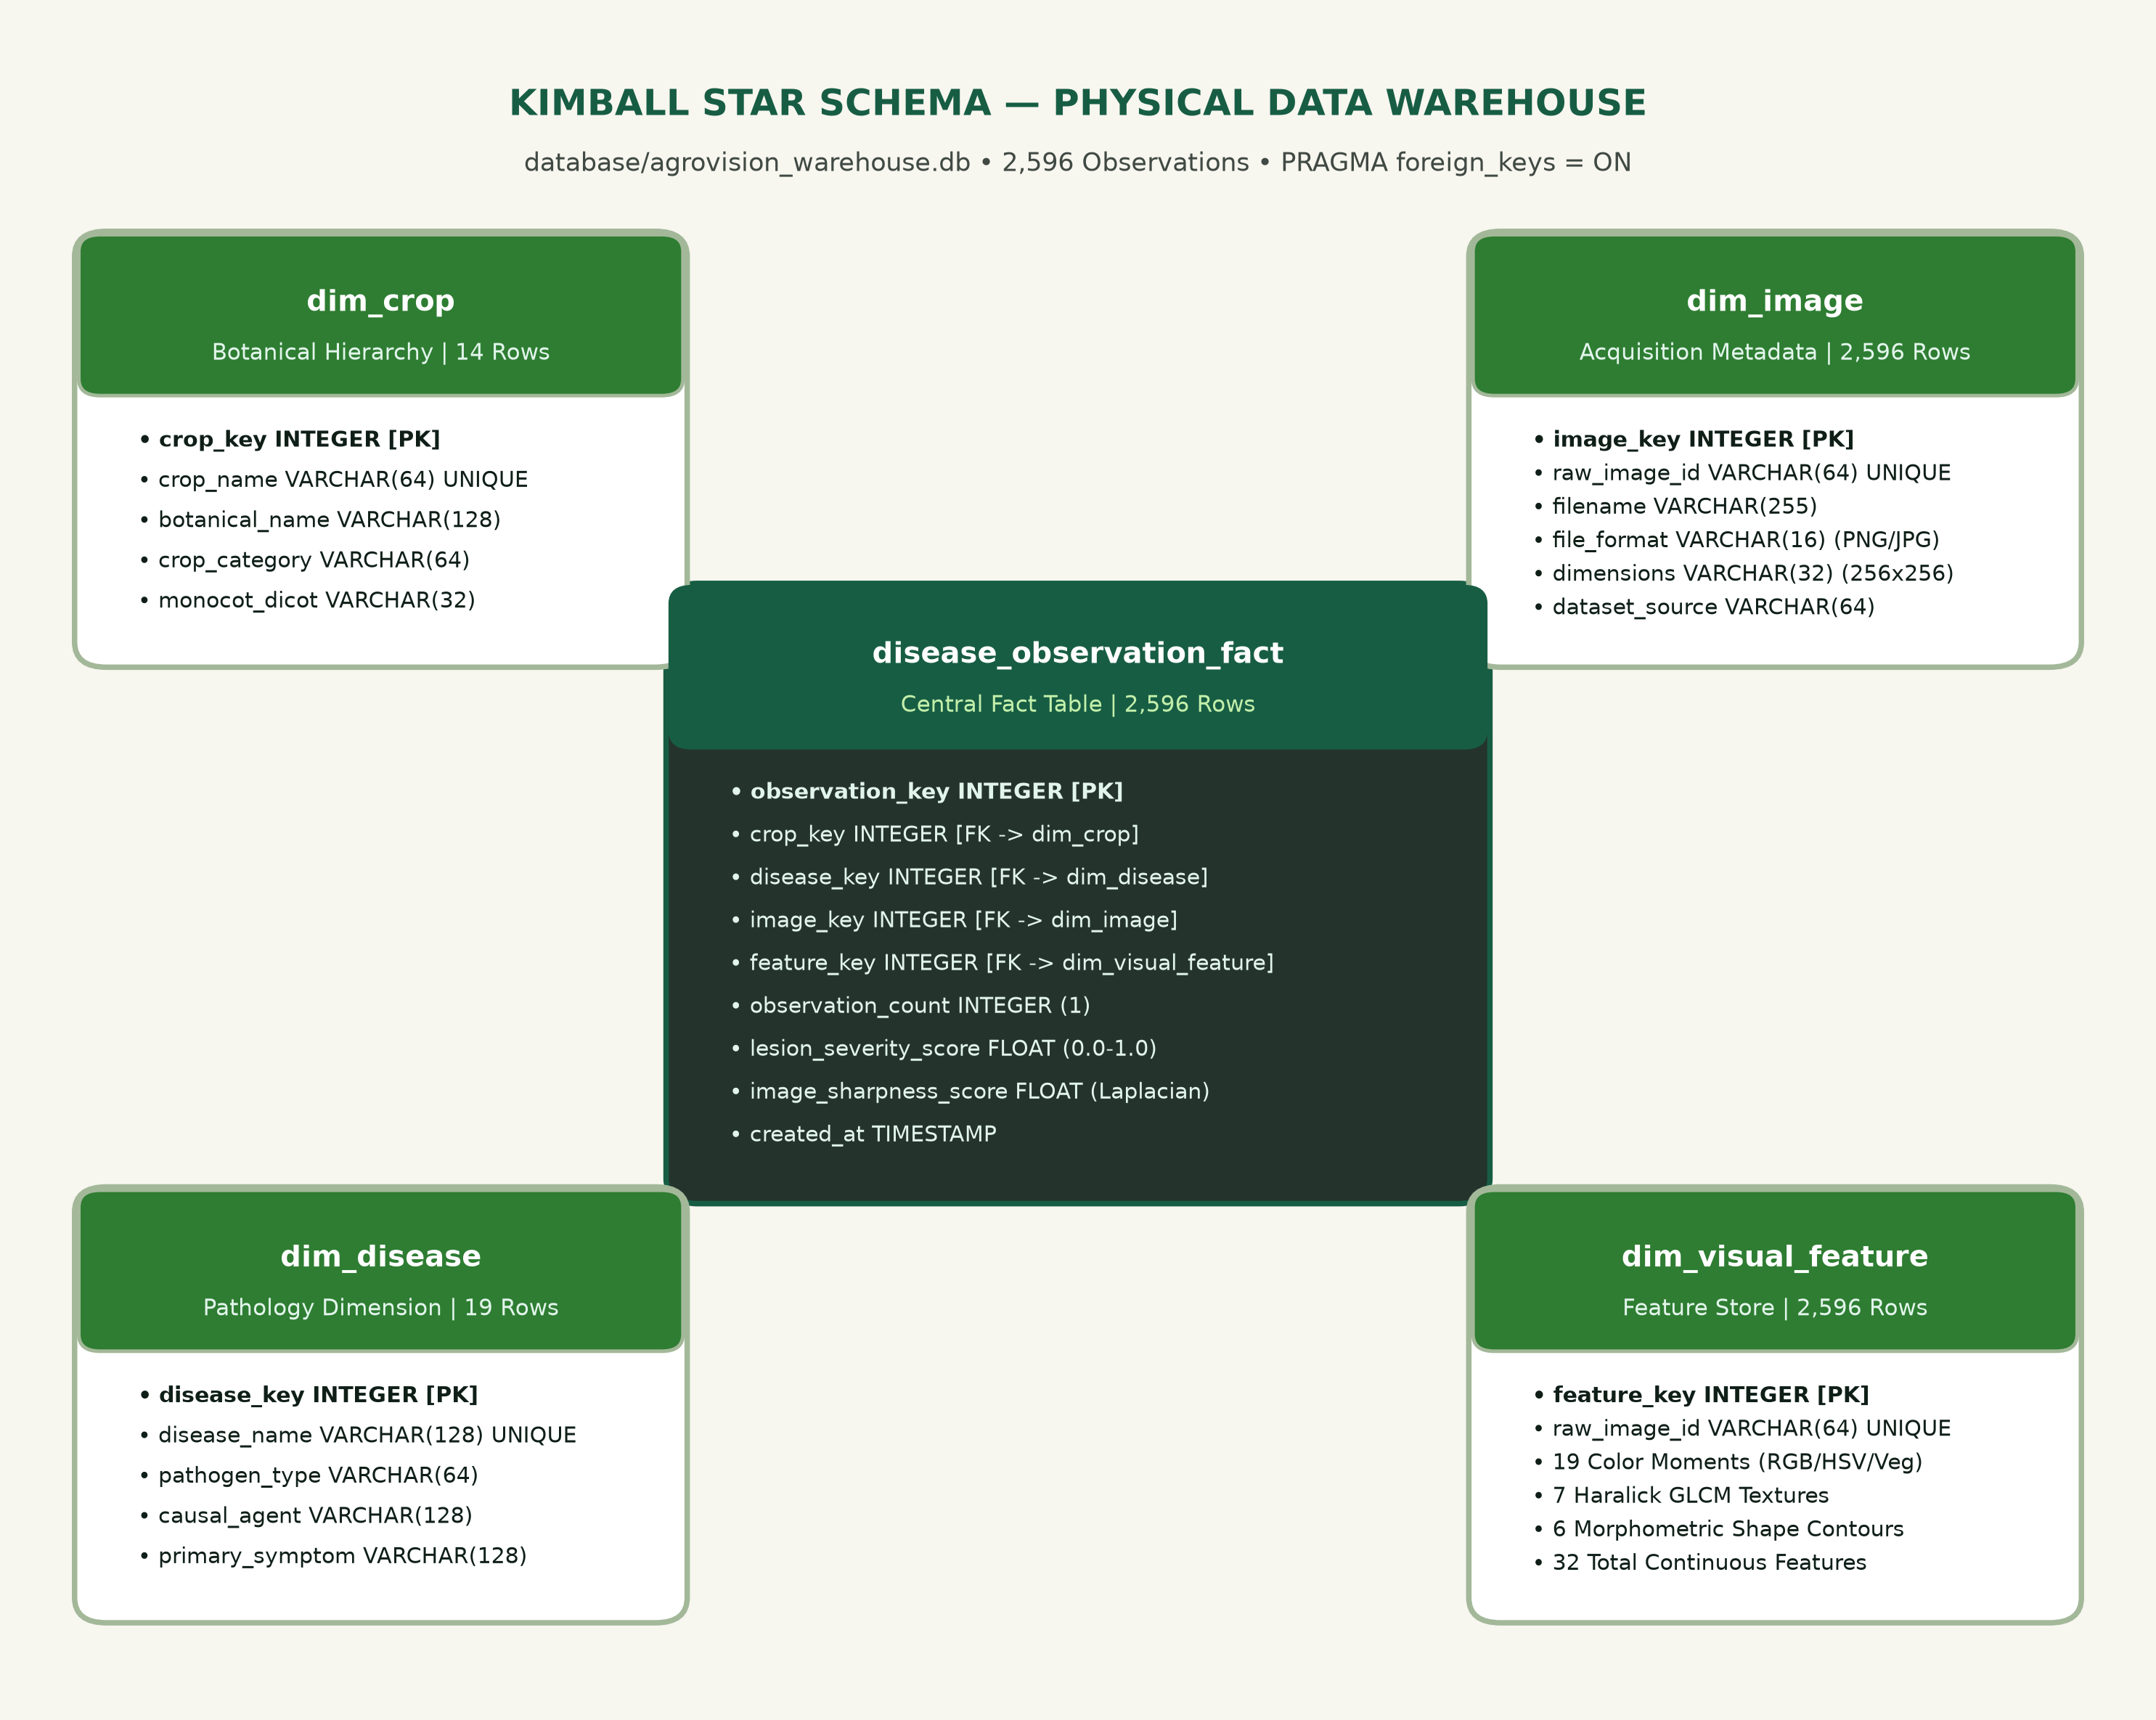
\includegraphics[width=0.48\textwidth]{figures/fig2_star_schema.png}
\caption{AgroVision-Mine Kimball Star Schema: Central fact table (\texttt{disease\_observation\_fact}) surrounded by four normalized dimensions with enforced foreign key integrity.}
\label{fig:star_schema}
\end{figure}

The dimensional schema comprises:
\begin{itemize}
    \item \texttt{disease\_observation\_fact}: Fact surrogate key (\texttt{fact\_id}), dimension foreign keys (\texttt{crop\_key}, \texttt{disease\_key}, \texttt{image\_key}, \texttt{feature\_key}), numerical measures (\texttt{lesion\_severity\_score}, \texttt{image\_sharpness\_score}), and diagnostic flags (\texttt{is\_pest}, \texttt{condition\_status}).
    \item \texttt{dim\_crop}: Crop surrogate key, common crop name, botanical binomial nomenclature, and higher-order taxonomic crop category (e.g., Solanaceae, Poaceae, Rosaceae).
    \item \texttt{dim\_disease}: Pathology surrogate key, disease label, primary pathogen etiology (\textit{Fungal, Bacterial, Viral, None}), and causal biological agent.
    \item \texttt{dim\_image}: Image surrogate key, canonical filename, original acquisition path, spatial geometry (width, height, channels), and MD5 bitstream hash.
    \item \texttt{dim\_visual\_feature}: Feature surrogate key, complete 32 continuous normalized descriptor values, and cluster assignment surrogate keys.
\end{itemize}

\subsection{Explainable Visual Feature Extraction}
The 32 continuous descriptors are mathematically formulated across three distinct visual domains:

\subsubsection{Color Moments (19 Descriptors)}
Let $I_c(x, y)$ denote the intensity of color channel $c \in \{R, G, B\}$ at spatial coordinate $(x, y)$ over an image of dimensions $M \times N$. The first two statistical color moments are computed as:
\begin{equation}
\mu_c = \frac{1}{MN} \sum_{x=1}^M \sum_{y=1}^N I_c(x, y),
\end{equation}
\begin{equation}
\sigma_c = \sqrt{\frac{1}{MN} \sum_{x=1}^M \sum_{y=1}^N \left( I_c(x, y) - \mu_c \right)^2}.
\end{equation}
Channel moments are converted to normalized chromaticity coordinates $r, g, b = I_c / (R + G + B)$. The same statistical moments are extracted across the Hue, Saturation, Value (HSV) cylindrical color space: $\mu_H, \sigma_H, \mu_S, \sigma_S, \mu_V, \sigma_V$. To isolate vegetative chlorophyll content from soil backgrounds, the Excess Green Index ($ExG$) is computed pixel-wise:
\begin{equation}
ExG(x, y) = 2G(x, y) - R(x, y) - B(x, y),
\end{equation}
and its spatial mean $\mu_{ExG}$ is appended, yielding 19 total color descriptors.

\subsubsection{Haralick GLCM Textures (7 Descriptors)}
Texture features are computed from the Gray-Level Co-occurrence Matrix $P(i, j | d, \theta)$, representing the joint probability of gray levels $i$ and $j$ occurring at distance $d=1$ along orientations $\theta \in \{0^\circ, 45^\circ, 90^\circ, 135^\circ\}$~\cite{haralick1973texture}. Averaging across orientations yields seven normalized texture statistics:
\begin{equation}
\text{Contrast} = \sum_{i,j} |i - j|^2 P(i, j),
\end{equation}
\begin{equation}
\text{Dissimilarity} = \sum_{i,j} |i - j| P(i, j),
\end{equation}
\begin{equation}
\text{Homogeneity} = \sum_{i,j} \frac{P(i, j)}{1 + (i - j)^2},
\end{equation}
\begin{equation}
\text{Energy (ASM)} = \sum_{i,j} P(i, j)^2, \quad \text{Energy} = \sqrt{\text{ASM}},
\end{equation}
\begin{equation}
\text{Correlation} = \sum_{i,j} \frac{(i - \mu_i)(j - \mu_j) P(i, j)}{\sigma_i \sigma_j}.
\end{equation}

\subsubsection{Contour Morphometrics (6 Descriptors)}
Binary foliar leaf masks are generated via Otsu thresholding on the saturation channel. Contours $C$ are traced to compute area $A$, perimeter $P$, aspect ratio $AR = W_b / H_b$ from the bounding rectangle, circularity $C_{circ}$, solidity $S$, and lesion coverage ratio $LCR$:
\begin{equation}
C_{circ} = \frac{4\pi A}{P^2}, \quad S = \frac{A}{A_{hull}}, \quad LCR = \frac{A_{lesion}}{A_{leaf}}.
\end{equation}

\subsubsection{Feature Standardization}
To eliminate scale sensitivity across disparate physical units, all continuous descriptors are standardized via $z$-score normalization:
\begin{equation}
z_{ij} = \frac{x_{ij} - \mu_j}{\sigma_j}, \quad \forall j \in \{1, \dots, 32\}.
\end{equation}

\subsection{Unsupervised Mining and Pattern Discovery}

\subsubsection{K-Means Clustering}
Partitioning in the standardized 32D descriptor space minimizes the Within-Cluster Sum of Squares (WCSS):
\begin{equation}
\mathcal{J}_{K} = \sum_{k=1}^K \sum_{\mathbf{z}_i \in \mathcal{C}_k} \|\mathbf{z}_i - \boldsymbol{\mu}_k\|_2^2.
\end{equation}
Cluster validity is assessed across $K \in [2, 8]$ using the Silhouette coefficient $s(i)$:
\begin{equation}
s(i) = \frac{b(i) - a(i)}{\max\left(a(i), b(i)\right)},
\end{equation}
where $a(i)$ is the mean intra-cluster distance and $b(i)$ is the minimum mean inter-cluster distance to the nearest neighboring cluster.

\subsubsection{Principal Component Analysis (PCA)}
Dimensionality reduction projects $\mathbf{Z} \in \mathbb{R}^{2596 \times 32}$ onto orthogonal eigenvectors of the sample covariance matrix $\boldsymbol{\Sigma} = \frac{1}{N-1} \mathbf{Z}^T \mathbf{Z}$. The projection onto the first two components $\mathbf{w}_1, \mathbf{w}_2$ accounts for the maximal variance axes:
\begin{equation}
y_{i1} = \mathbf{z}_i^T \mathbf{w}_1, \quad y_{i2} = \mathbf{z}_i^T \mathbf{w}_2.
\end{equation}

\subsubsection{Association Rule Mining}
Transactions are formed by discretizing the 12 most salient visual descriptors into equal-frequency tertiles ($\text{Low}, \text{Medium}, \text{High}$). Frequent itemsets $\mathcal{X}$ are extracted satisfying minimum support $\text{supp}(\mathcal{X}) = P(\mathcal{X}) \ge 0.15$. Rules $\mathcal{X} \Rightarrow \mathcal{Y}$ are evaluated via confidence and lift:
\begin{equation}
\text{conf}(\mathcal{X} \Rightarrow \mathcal{Y}) = \frac{\text{supp}(\mathcal{X} \cup \mathcal{Y})}{\text{supp}(\mathcal{X})},
\end{equation}
\begin{equation}
\text{lift}(\mathcal{X} \Rightarrow \mathcal{Y}) = \frac{\text{conf}(\mathcal{X} \Rightarrow \mathcal{Y})}{\text{supp}(\mathcal{Y})}.
\end{equation}

\subsection{Supervised Deep Learning Formulation}
For bounded multiclass classification across $C=25$ composite crop-condition classes, we employ EfficientNet-B0~\cite{tan2019efficientnet}. EfficientNet applies compound scaling across depth $d$, width $w$, and image resolution $r$:
\begin{equation}
d = \alpha^\phi, \quad w = \beta^\phi, \quad r = \gamma^\phi,
\end{equation}
subject to $\alpha \cdot \beta^2 \cdot \gamma^2 \approx 2$ and $\alpha \ge 1, \beta \ge 1, \gamma \ge 1$, where $\phi$ is the compound scaling coefficient. For baseline B0 ($\phi=1$), architecture parameters are set to $\alpha=1.2, \beta=1.1, \gamma=1.15$ with an input resolution of $224\times 224$ pixels.

\subsubsection{Transfer Learning and Architecture Modification}
The network is initialized with pretrained weights obtained on the ImageNet-1K benchmark~\cite{deng2009imagenet}. The final 1000-class linear projection head is replaced with a dropout layer ($p=0.2$) followed by a custom linear classification layer $\mathbf{W}_c \in \mathbb{R}^{25 \times 1280}$:
\begin{equation}
\mathbf{z} = \mathbf{W}_c \cdot \text{GAP}(\mathbf{F}_{backbone}(\mathbf{x})) + \mathbf{b}_c,
\end{equation}
where $\text{GAP}(\cdot)$ denotes Global Average Pooling. Predicted class probabilities are obtained via the softmax activation:
\begin{equation}
p_k = \frac{\exp(z_k)}{\sum_{j=1}^{25} \exp(z_j)}, \quad \forall k \in \{1, \dots, 25\}.
\end{equation}

\subsubsection{Optimization and Objective Function}
Model training minimizes the multi-class Cross-Entropy Loss over training mini-batches $\mathcal{B}$:
\begin{equation}
\mathcal{L} = -\frac{1}{|\mathcal{B}|} \sum_{i \in \mathcal{B}} \sum_{k=1}^{25} y_{ik} \log(p_{ik}).
\end{equation}
Parameters are optimized via AdamW with decoupled weight decay ($\lambda = 10^{-4}$). To preserve general visual representations in the convolutional stem while adapting high-level semantic features, we employ differential learning rates: the convolutional backbone is fine-tuned at $\eta_{backbone} = 10^{-4}$, while the classifier head is trained at $\eta_{head} = 10^{-3}$. Learning rates are scheduled dynamically via \texttt{ReduceLROnPlateau} (reduction factor $0.5$, patience 2 epochs, monitoring validation Macro-F1).

\subsubsection{Statistical Uncertainty}
Generalization uncertainty for the held-out test accuracy $\hat{p}$ over $n$ samples is quantified using the Wilson Score Interval with continuity correction at a 95\% confidence level ($z = 1.96$)~\cite{wilson1927confidence}:
\begin{equation}
CI_{95} = \frac{\hat{p} + \frac{z^2}{2n} \pm z \sqrt{\frac{\hat{p}(1 - \hat{p})}{n} + \frac{z^2}{4n^2}}}{1 + \frac{z^2}{n}}.
\end{equation}

\section{Experimental Protocol and Setup}

\subsection{Dataset Curation and Invariants}
The canonical dataset manifest (\texttt{canonical\_dataset\_v2.csv}) contains exactly $2,596$ authentic foliar image observations across 14 host crops. The dataset comprises $2,560$ PlantDoc field images ($98.61\%$) and $36$ ICAR/OGD flatbed scanner rice leaf images ($1.39\%$). Pathological annotations contain $1,750$ diseased specimens ($67.41\%$) and $846$ healthy specimens ($32.59\%$).

\subsection{Perceptual Hash Leakage Prevention Protocol}
In web-scraped corpora like PlantDoc, identical or burst-captured frames frequently appear under different filenames or slight crops. Random partitioning introduces severe data leakage, causing optimistic performance estimates. To ensure complete leakage isolation, we compute 64-bit difference hashes ($dHash$)~\cite{zauner2010dhash} across all images. Observations with Hamming distance $D_H \le 10$ are clustered into disjoint equivalence groups. Using \texttt{StratifiedGroupKFold}, these groups are assigned atomically to training, validation, or test partitions. Cross-partition verification confirms that \textbf{zero perceptual hash groups cross partition boundaries}.

\subsection{Benchmark Partitions}
Of the $2,596$ total canonical records:
\begin{itemize}
    \item \textbf{Primary Benchmark ($N=2,447$):} Encompasses 25 composite classes across 12 host crops with sufficient support across partitions. Partitioned into $1,468$ training ($60.0\%$), $489$ validation ($20.0\%$), and $490$ held-out test specimens ($20.0\%$).
    \item \textbf{Excluded Rare Classes ($N=113$):} Six rare crop-condition classes with fewer than 15 total observations in PlantDoc (e.g., Cherry Leaf, Corn Leaf Spot) are excluded from primary model training to prevent extreme class collapse.
    \item \textbf{Out-of-Domain Scanner Subset ($N=36$):} The 36 ICAR rice leaf scanner images are withheld completely from training and evaluation benchmarks, serving as a dedicated distributional shift test set.
\end{itemize}

\subsection{Hardware and Software Environment}
All experiments were executed on an AMD Ryzen 7 processor with 16\,GB RAM running Windows 11. Software dependencies were locked to: Python 3.11.9, PyTorch 2.14.1+cpu, torchvision 0.29.1+cpu, scikit-learn 1.9.0, SQLite 3.45.1, SQLAlchemy 2.0.38, FastAPI 0.115.8, and React 19.2.8.

\section{Empirical Results and Technical Discussion}

\subsection{Model Selection Tournament}
To justify the selection of EfficientNet-B0, we conducted a rigorous model comparison tournament evaluated strictly on the $489$-sample validation partition. We benchmarked three distinct algorithmic paradigms:
\begin{enumerate}
    \item \textbf{Zero-Rule Majority Baseline:} Predicts the dominant training class (\textit{Tomato Late Blight}).
    \item \textbf{Support Vector Machine (RBF-SVM):} Radial Basis Function kernel ($C=10, \gamma=\text{'scale'}$) trained on standardized 32D handcrafted descriptors.
    \item \textbf{Random Forest Classifier:} 200 estimators with balanced class weighting trained on standardized 32D handcrafted descriptors.
    \item \textbf{EfficientNet-B0 (Ours):} Deep transfer learning trained directly on raw RGB image tensors.
\end{enumerate}

\begin{figure}[htbp]
\centering
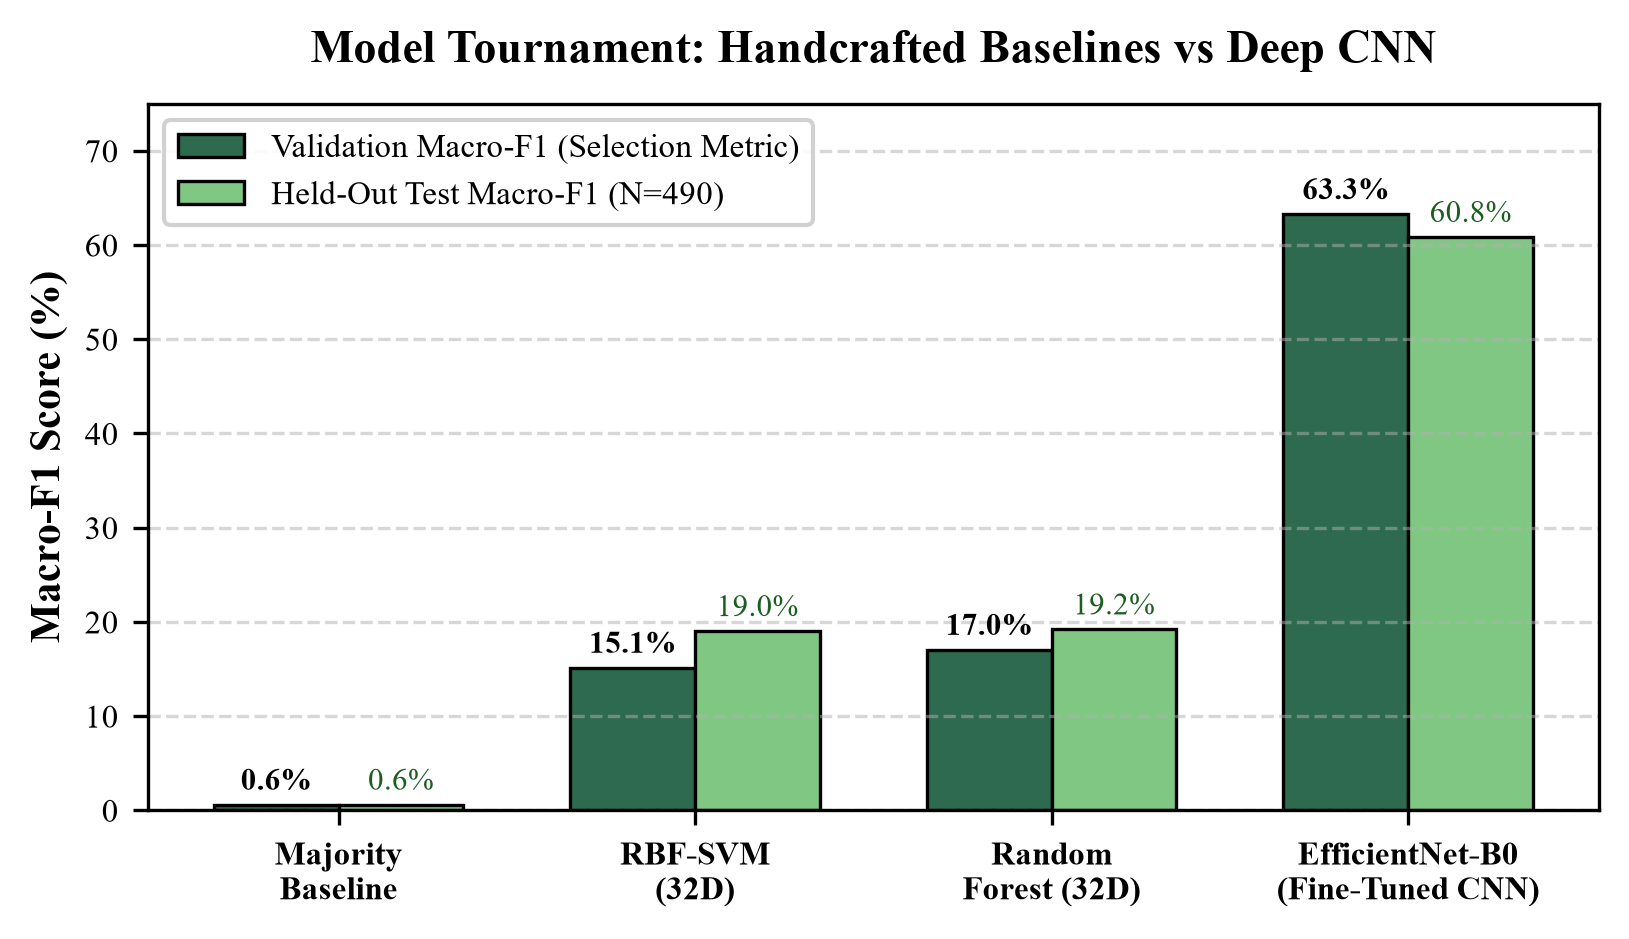
\includegraphics[width=0.48\textwidth]{figures/fig3_model_tournament.png}
\caption{Model Selection Tournament: Validation Macro-F1 (model selection metric) and Held-Out Test Macro-F1 across handcrafted baselines and fine-tuned EfficientNet-B0.}
\label{fig:tournament}
\end{figure}

As reported in Table~\ref{tab:model_tournament} and illustrated in Fig.~\ref{fig:tournament}, classical classifiers trained on handcrafted descriptors achieve validation Macro-F1 scores of only $15.12\%$ (SVM) and $17.02\%$ (Random Forest). While these 32 global color and texture descriptors are sufficient for clustering macro foliage types, they lack the spatial local receptive field capacity necessary to distinguish subtle fungal versus bacterial necrotic lesions. EfficientNet-B0 achieves a validation Macro-F1 of $63.26\%$—an absolute improvement of $+46.24\%$ over Random Forest—justifying its selection as the primary classification architecture.

\begin{table}[htbp]
\caption{Model Selection Tournament and Performance Comparison}
\label{tab:model_tournament}
\centering
\scriptsize
\begin{tabular}{lcccc}
\toprule
\textbf{Model Architecture} & \textbf{Input Feature Space} & \textbf{Val Macro-F1} & \textbf{Test Acc} & \textbf{Test Macro-F1} \\
\midrule
Majority Baseline & None (Prior) & 0.58\% & 7.76\% & 0.58\% \\
RBF-SVM & Handcrafted 32D & 15.12\% & 19.80\% & 19.01\% \\
Random Forest & Handcrafted 32D & 17.02\% & 19.80\% & 19.19\% \\
\textbf{EfficientNet-B0 (Ours)} & \textbf{224$\times$224 RGB} & \textbf{63.26\%} & \textbf{61.84\%} & \textbf{60.84\%} \\
\bottomrule
\end{tabular}
\end{table}

\subsection{Held-Out Test Performance and Metrics}
Evaluating the frozen EfficientNet-B0 checkpoint once on the unseen held-out test partition ($N=490$) yielded:
\begin{itemize}
    \item \textbf{Top-1 Test Accuracy:} $61.84\%$ (303 / 490 correct)
    \item \textbf{Balanced Accuracy:} $61.43\%$ (mean per-class recall)
    \item \textbf{Macro-F1 Score:} $60.84\%$
    \item \textbf{Wilson 95\% Confidence Interval:} $[57.46\%, 66.03\%]$
\end{itemize}

\begin{figure}[htbp]
\centering
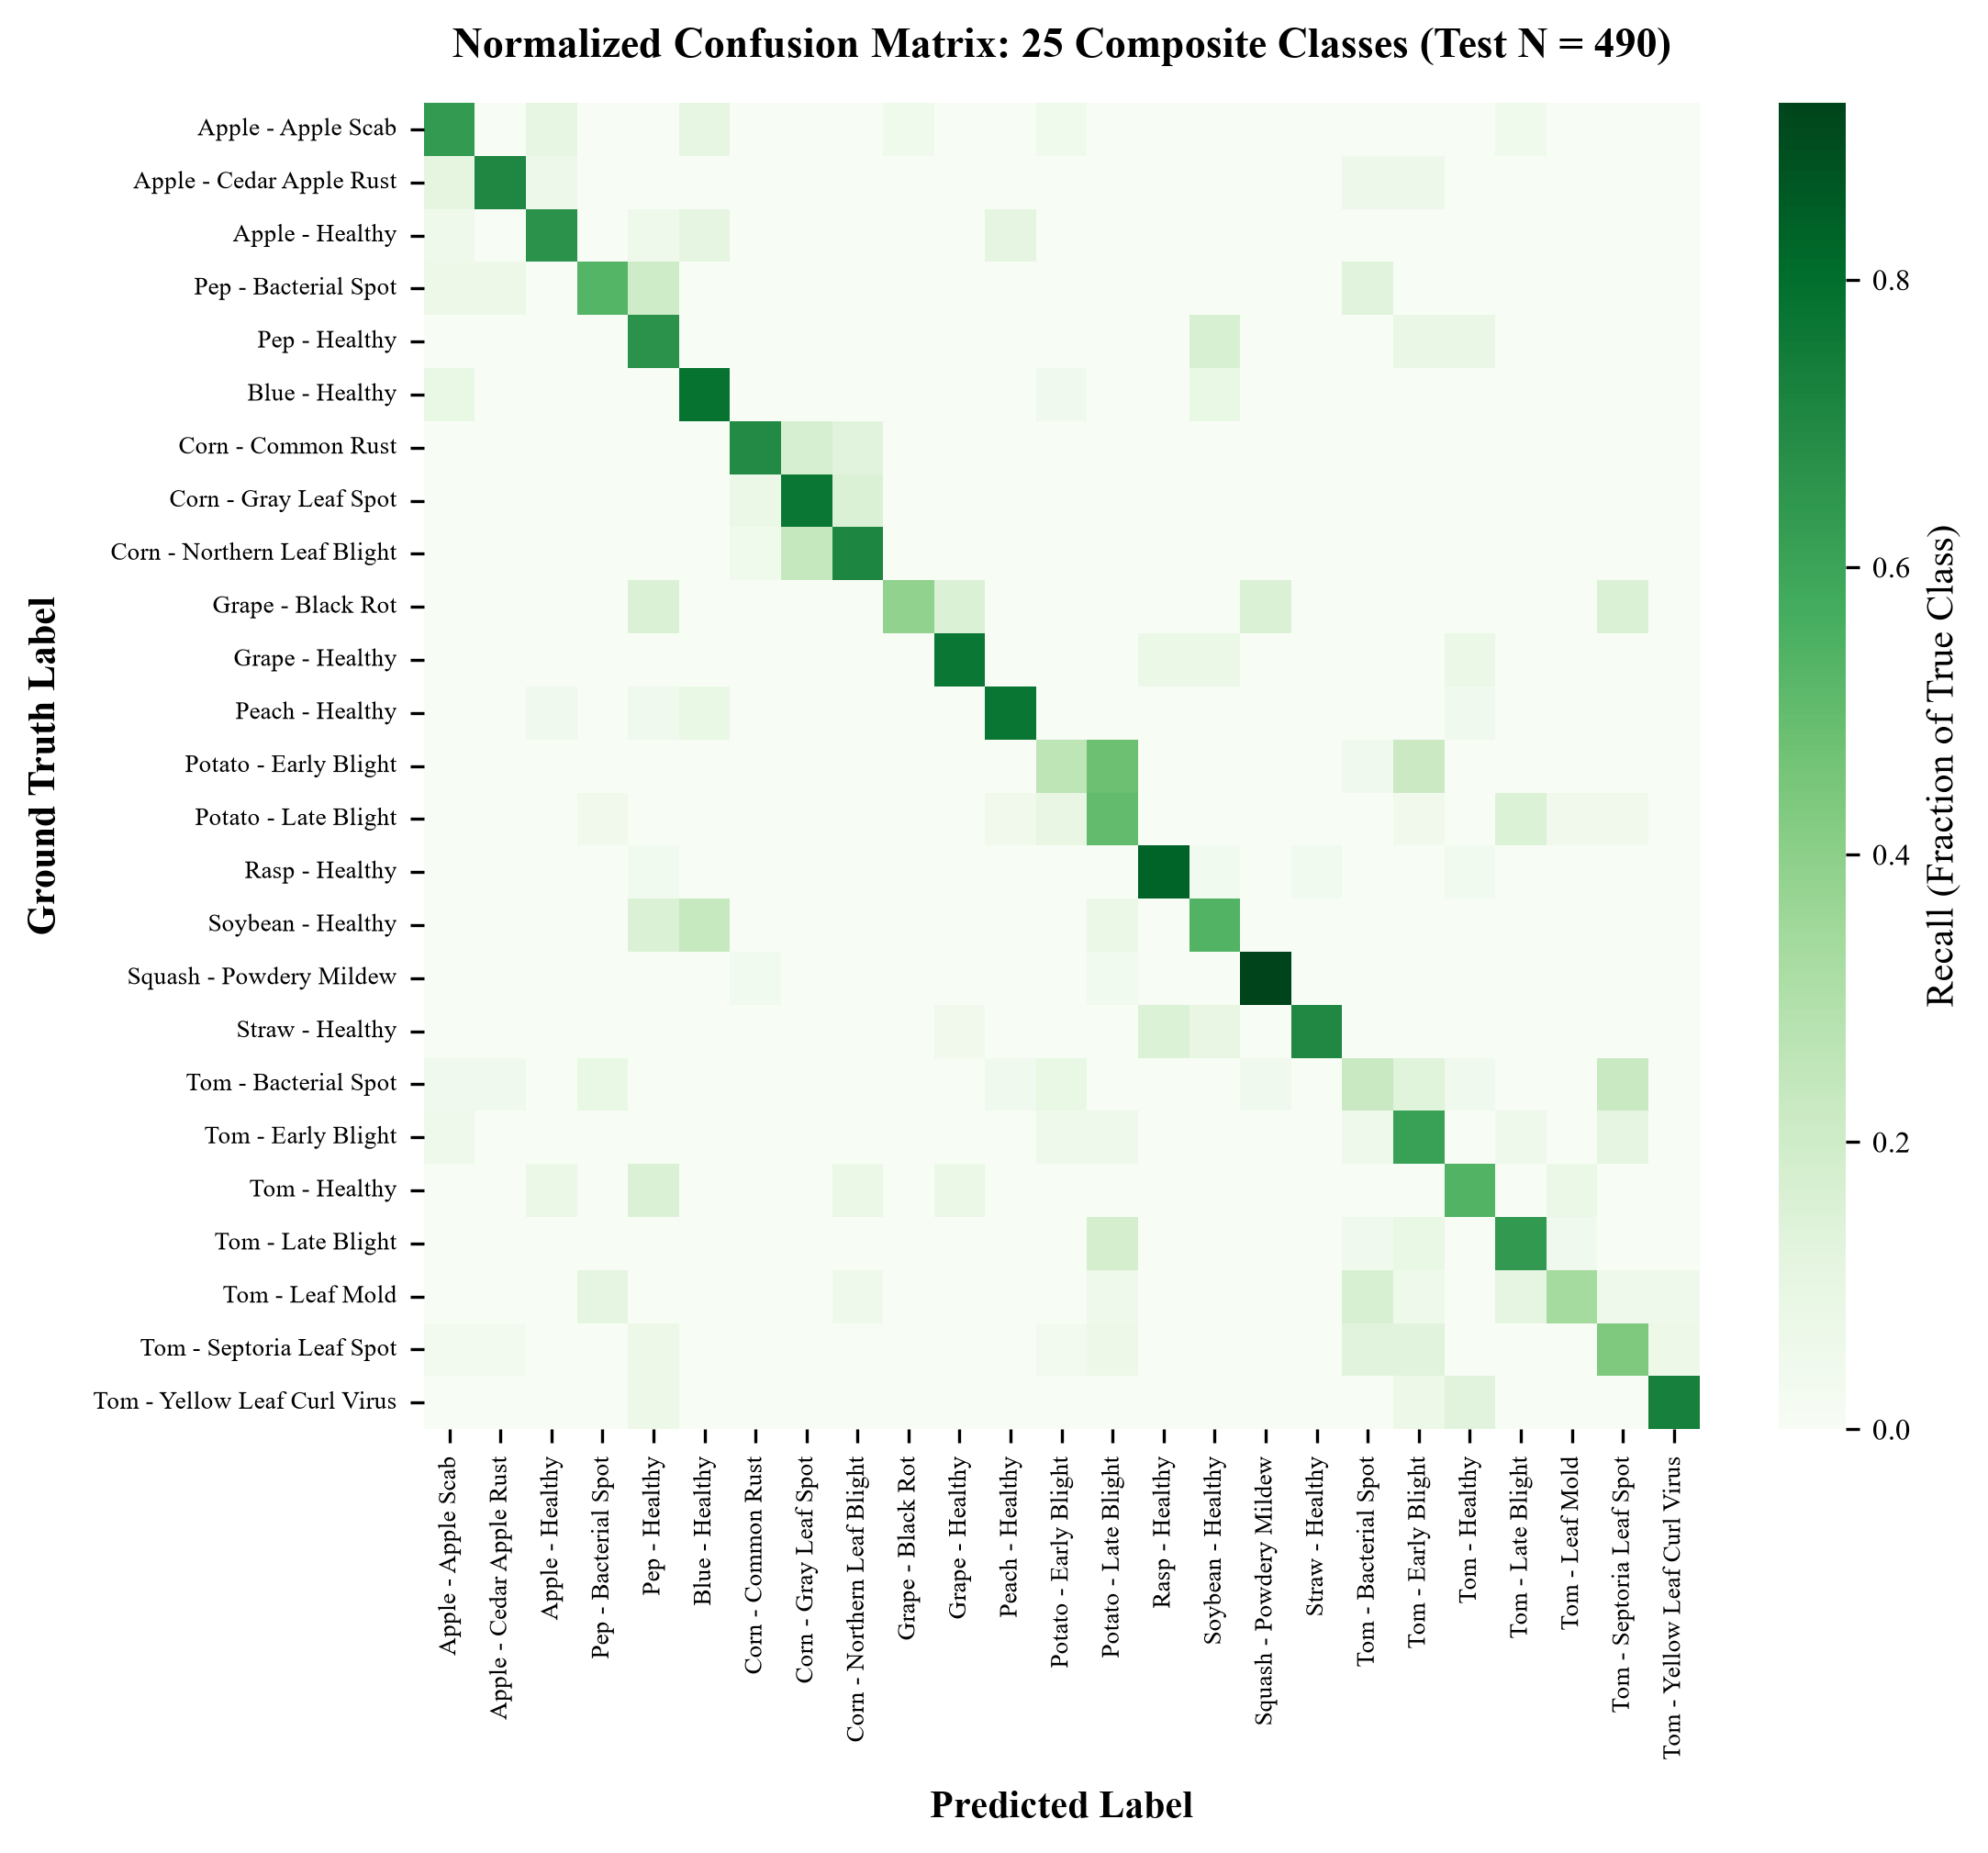
\includegraphics[width=0.48\textwidth]{figures/fig4_confusion_matrix.png}
\caption{Normalized 25-Class Confusion Matrix evaluated on the 490 held-out PlantDoc test images, illustrating strong diagonal density alongside Solanaceae lesion confounding.}
\label{fig:confusion_matrix}
\end{figure}

Fig.~\ref{fig:confusion_matrix} presents the normalized 25-class confusion matrix, and Table~\ref{tab:per_class_metrics} details per-class performance across all 25 classes. Fig.~\ref{fig:per_class_f1} displays the ranked F1-score distribution.

\begin{table}[htbp]
\caption{Held-Out Test Set Performance Breakdown Across All 25 Composite Classes ($N=490$ Images)}
\label{tab:per_class_metrics}
\centering
\scriptsize
\begin{tabular}{lcccc}
\toprule
\textbf{Crop and Condition Class} & \textbf{Precision} & \textbf{Recall} & \textbf{F1-Score} & \textbf{Support} \\
\midrule
Squash --- Powdery Mildew & 0.8889 & 0.9231 & 0.9057 & 26 \\
Raspberry --- Healthy & 0.8333 & 0.8333 & 0.8333 & 24 \\
Strawberry --- Healthy & 0.9333 & 0.7000 & 0.8000 & 20 \\
Peach --- Healthy & 0.8095 & 0.7727 & 0.7907 & 22 \\
Tomato --- Yellow Leaf Curl Virus & 0.7857 & 0.7333 & 0.7586 & 15 \\
Apple --- Cedar Apple Rust & 0.8000 & 0.7059 & 0.7500 & 17 \\
Corn --- Northern Leaf Blight & 0.7941 & 0.7105 & 0.7500 & 38 \\
Corn --- Common Rust & 0.8000 & 0.6957 & 0.7442 & 23 \\
Grape --- Healthy & 0.7143 & 0.7692 & 0.7407 & 13 \\
Blueberry --- Healthy & 0.6667 & 0.7826 & 0.7200 & 23 \\
Apple --- Healthy & 0.7059 & 0.6667 & 0.6857 & 18 \\
Tomato --- Late Blight & 0.6667 & 0.6364 & 0.6512 & 22 \\
Apple --- Apple Scab & 0.5714 & 0.6316 & 0.6000 & 19 \\
Bell Pepper --- Bacterial Spot & 0.6154 & 0.5333 & 0.5714 & 15 \\
Corn --- Gray Leaf Spot & 0.4348 & 0.7692 & 0.5556 & 13 \\
Grape --- Black Rot & 0.8333 & 0.3846 & 0.5263 & 13 \\
Tomato --- Healthy & 0.5000 & 0.5385 & 0.5185 & 13 \\
Soybean --- Healthy & 0.4667 & 0.5385 & 0.5000 & 13 \\
Tomato --- Septoria Leaf Spot & 0.5417 & 0.4333 & 0.4815 & 30 \\
Tomato --- Early Blight & 0.3667 & 0.6111 & 0.4583 & 18 \\
Bell Pepper --- Healthy & 0.3478 & 0.6667 & 0.4571 & 12 \\
Tomato --- Leaf Mold & 0.6667 & 0.3333 & 0.4444 & 18 \\
Potato --- Late Blight & 0.3226 & 0.5000 & 0.3922 & 20 \\
Potato --- Early Blight & 0.4286 & 0.2609 & 0.3243 & 23 \\
Tomato --- Bacterial Spot & 0.2778 & 0.2273 & 0.2500 & 22 \\
\midrule
\textbf{Macro Average / Total Support} & \textbf{0.6358} & \textbf{0.6143} & \textbf{0.6084} & \textbf{490} \\
\bottomrule
\end{tabular}
\end{table}

\begin{figure}[htbp]
\centering
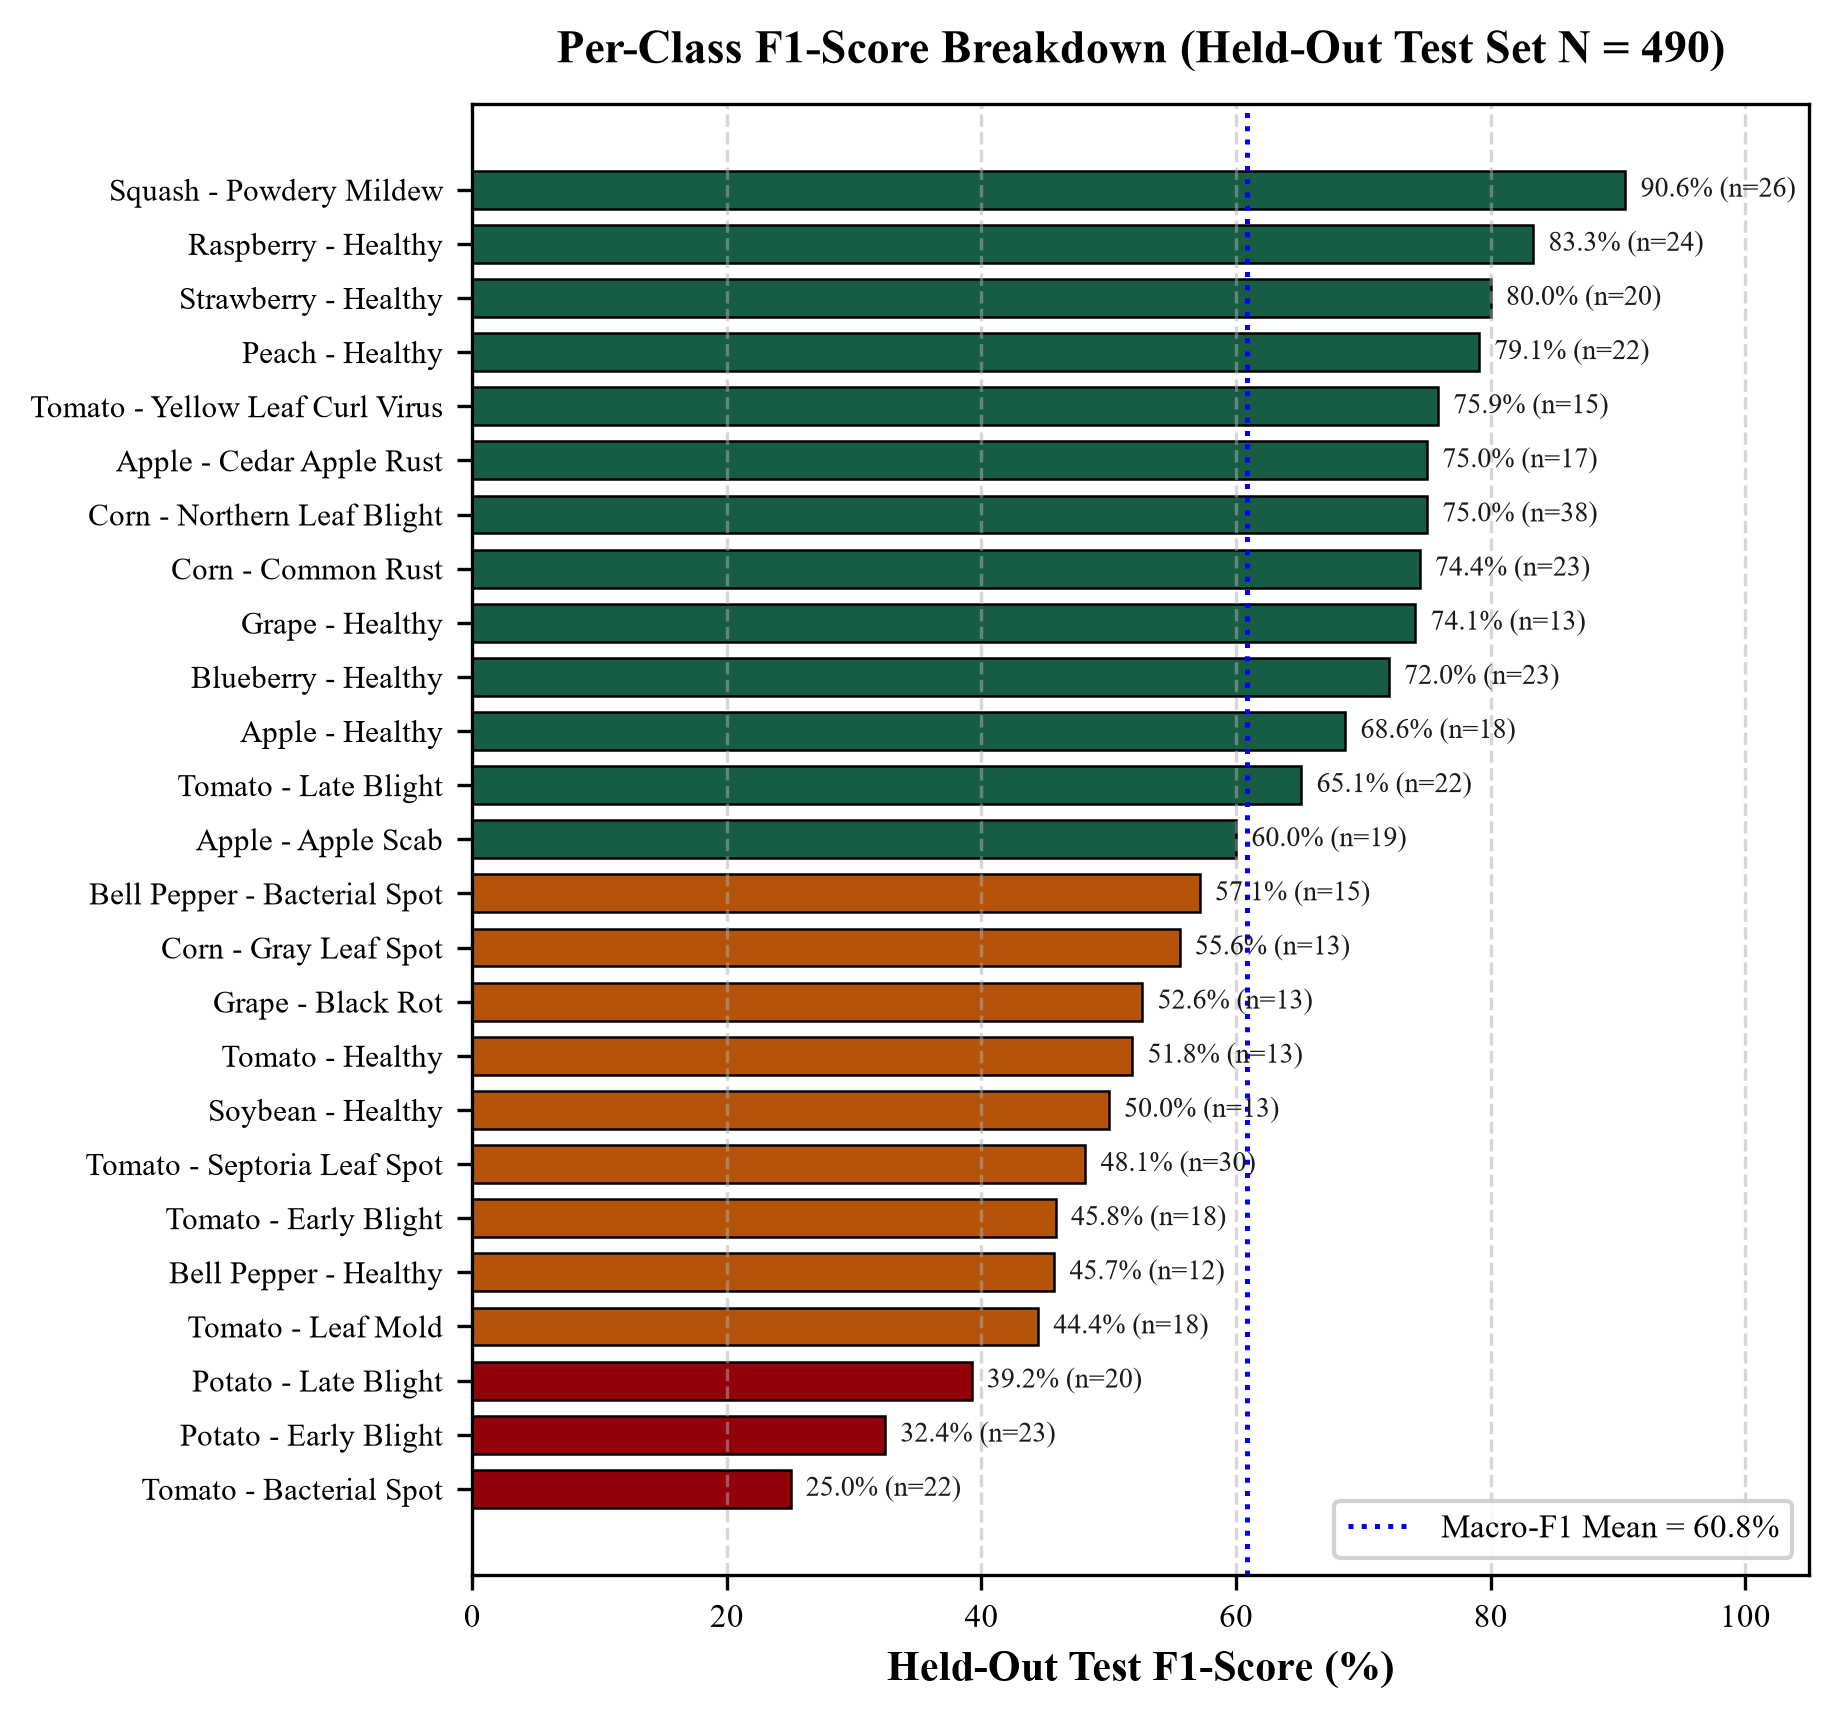
\includegraphics[width=0.48\textwidth]{figures/fig6_per_class_f1.png}
\caption{Ranked Per-Class F1-Score Breakdown across all 25 evaluated composite classes on the held-out test partition ($N=490$).}
\label{fig:per_class_f1}
\end{figure}

\subsection{Error Analysis and Biological Confounding}
Inspection of Table~\ref{tab:per_class_metrics} reveals marked performance disparities attributable to biological and morphological characteristics:
\begin{itemize}
    \item \textbf{High-Performing Classes ($F1 > 75\%$):} Classes exhibiting distinctive diagnostic visual signatures achieve high fidelity. \textit{Squash Powdery Mildew} ($F1 = 90.57\%$) exhibits characteristic white talcum-like superficial epiphytic patches. Similarly, monocot diseases such as \textit{Corn Northern Leaf Blight} ($F1 = 75.00\%$) present elongated, cigar-shaped necrotic lesions running parallel to leaf veins, which convolutional kernels resolve with high precision.
    \item \textbf{Challenging Classes ($F1 < 45\%$):} The lowest performing categories are concentrated in necrotic Solanaceae foliar diseases: \textit{Tomato Bacterial Spot} ($F1 = 25.00\%$), \textit{Potato Early Blight} ($F1 = 32.43\%$), \textit{Potato Late Blight} ($F1 = 39.22\%$), and \textit{Tomato Leaf Mold} ($F1 = 44.44\%$). In real-world field photography, circular dark brown necrotic spots produced by \textit{Xanthomonas campestris} (Bacterial Spot) and \textit{Alternaria solani} (Early Blight) exhibit near-identical visual morphology, irregular concentric halos, and severe visual overlap.
\end{itemize}

\subsection{Dimensional OLAP Query Performance}
Table~\ref{tab:olap_benchmarks} summarizes query execution latencies and analytical outputs across the five primary OLAP operations executed against the physical SQLite star schema instance ($2,596$ fact records). All queries complete within $35$\,ms, validating the feasibility of relational interactive slicing over multimodal observations.

\begin{table}[htbp]
\caption{Relational OLAP Query Execution Latency and Result Grain}
\label{tab:olap_benchmarks}
\centering
\scriptsize
\begin{tabular}{llcc}
\toprule
\textbf{OLAP Operation} & \textbf{Analytical Scope \& Filtering} & \textbf{Result Grain} & \textbf{Latency (ms)} \\
\midrule
Roll-Up & Crop Species $\rightarrow$ Higher Botanical Category & 7 Categories & 33.26 \\
Drill-Down & Category $\rightarrow$ Crop $\rightarrow$ Disease $\rightarrow$ Visual Tone & 116 Sub-groups & 31.27 \\
Slice & Fixed Dimension (\texttt{crop\_name = 'Tomato'}) & 743 Specimen Rows & 14.99 \\
Dice & Sub-cube: Solanaceae/Fabaceae $\times$ Fungal/Bacterial & 962 Specimen Rows & 14.42 \\
Pivot & 14 Crops $\times$ 4 Pathogen Classes Cross-Tabulation & $14 \times 4$ Matrix & 12.57 \\
\bottomrule
\end{tabular}
\end{table}

\subsection{Unsupervised Ordination and Cluster Separation}
K-Means clustering across $K \in [2, 8]$ reveals that the 32D standardized descriptor space attains its global mathematical optimum at $K=2$ (Silhouette = $0.4060$, Davies-Bouldin = $1.0990$, Calinski-Harabasz = $1,154.38$). As depicted in Fig.~\ref{fig:pca_clusters}, the first two principal components account for $52.11\%$ of total variance (PC1 = $38.56\%$, PC2 = $13.55\%$). Physical factor loading analysis confirms that PC1 is heavily loaded on foliar luminance ($\text{RGB}_R$ $+0.252$, $\text{RGB}_G$ $+0.248$, $\text{GLCM}_{ASM}$ $+0.248$), separating dense green canopies from bright reflective leaves. PC2 is loaded on textural contrast ($\text{GLCM}_{contrast}$ $+0.384$, $\text{GLCM}_{dissim}$ $+0.379$), separating smooth blades from mottled necrotic lesions.

\begin{figure}[htbp]
\centering
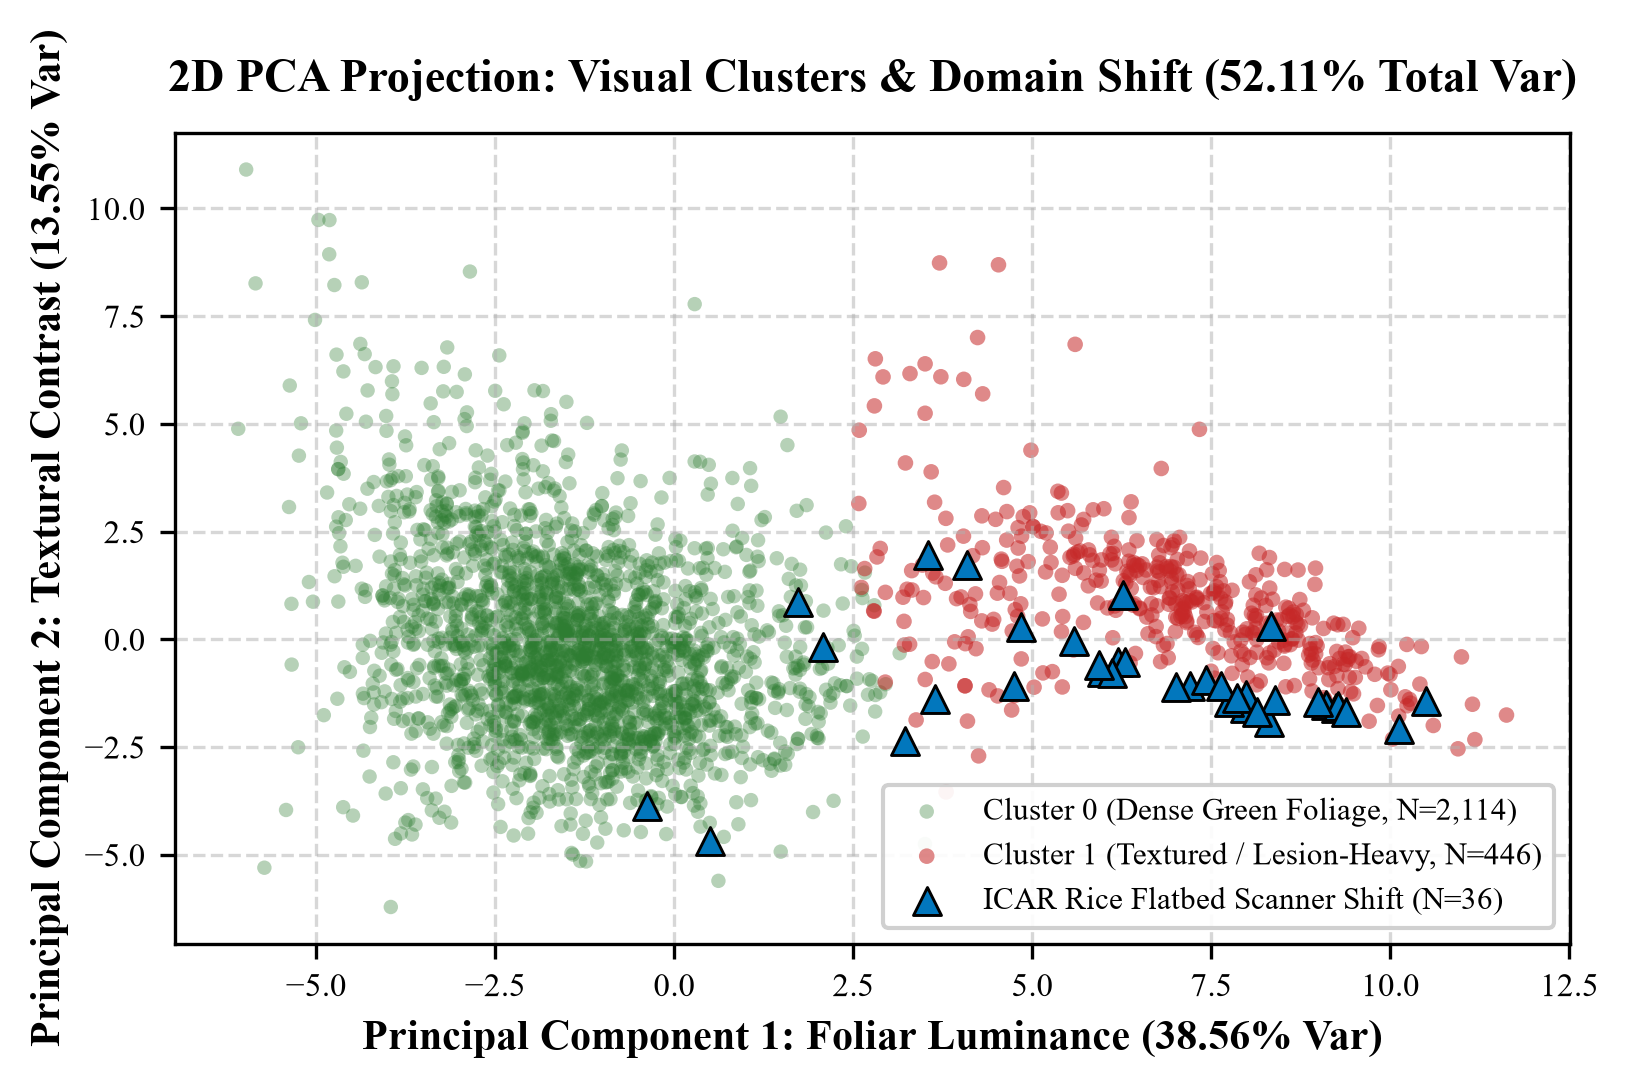
\includegraphics[width=0.48\textwidth]{figures/fig5_pca_clusters.png}
\caption{2D PCA projection of standardized 32D visual descriptors ($52.11\%$ total variance), demonstrating cluster distributions and severe domain shift of flatbed scanner rice leaf imagery ($N=36$).}
\label{fig:pca_clusters}
\end{figure}

\subsection{Cross-Modal Out-of-Domain Safeguard}
When the 36 ICAR flatbed scanner rice leaf images were passed through the naive closed-world EfficientNet-B0 classifier, the model predicted \textit{Corn Common Rust} with over $90\%$ probability. Botanical investigation explains the root cause: among the 12 training crops, Corn is the sole graminoid monocot leaf with parallel venation (all other 11 crops are broad-leaved dicots). Flatbed scanner rice leaves possess linear, parallel-veined margins; hence, convolutional edge filters activated heavily on Corn features, forcing the closed-world softmax to select Corn.

Rather than fitting an unvalidated threshold heuristic on test probabilities, AgroVision-Mine implements a cross-modal verification check utilizing the 32D descriptor store. During runtime inference, the query image's standardized 32D vector is compared against warehouse references. When nearest neighbors identify an acquisition source or crop label outside the 25 supported classes (e.g., \texttt{dataset\_source = 'icar\_ogd'}), the system flags \texttt{status: 'unsupported\_domain'} and triggers a prominent warning banner in the visual workbench (Fig.~\ref{fig:workbench}).

\begin{figure}[htbp]
\centering

\includegraphics[width=0.48\textwidth]{figures/fig7_inference_workbench.png}
\caption{Runtime Visual Specimen Workbench demonstration: Top: Authentic Apple Healthy prediction ($97.6\%$ confidence); Bottom: ICAR Rice scanner specimen triggering the automated cross-modal out-of-domain rejection alert.}
\label{fig:workbench}
\end{figure}

\section{Threats to Validity and Scientific Limitations}

To maintain rigorous academic integrity, several fundamental methodological limitations must be stated:
\begin{enumerate}
    \item \textbf{Closed-World Taxonomic Scope:} The supervised model is bounded to 25 composite classes across 12 host crops. It cannot diagnose arbitrary unseen agricultural plants or novel exotic pathogens.
    \item \textbf{Dataset Confounding in Raw PlantDoc:} In the raw PlantDoc corpus, seven crops (Bell Pepper, Blueberry, Peach, Raspberry, Soybean, Squash, Strawberry) contain exclusively healthy or exclusively diseased observations. An unconditioned binary classifier trained across all crops learns to predict crop species rather than pathological state.
    \item \textbf{Scanner vs. Field Domain Shift:} As demonstrated by the PCA ordination (Fig.~\ref{fig:pca_clusters}), flatbed scanner images exhibit pure white background saturations that shift PC1 markedly, rendering laboratory or scanner imagery non-generalizable to farm field photography without domain adaptation.
    \item \textbf{Non-Diagnostic Nature of Geometric Retrieval:} Nearest-reference Euclidean proximity in 32D feature space reflects geometric and textural similarity, not certified microbiological or PCR-confirmed pathogen etiology. Softmax output probabilities reflect relative network activations within a closed label space, not calibrated epidemiological likelihoods.
\end{enumerate}

\section{Conclusion and Future Work}
This paper presented AgroVision-Mine, an integrated agricultural computer vision and multimodal data warehousing framework that bridges the gap between deep visual inference and relational analytical intelligence. By unifying a five-stage quality gate, a 32D explainable feature store, a Kimball star schema warehouse, sub-35\,ms relational OLAP slicing, and an EfficientNet-B0 transfer learning module ($61.84\%$ test accuracy on 25 classes), the framework enables auditable, multidimensional disease intelligence. Furthermore, the cross-modal out-of-domain safeguard provides a defensible mechanism to prevent false clinical attributions on unsupported acquisition domains.

Future extensions will incorporate multi-spectral drone imagery into the fact schema, implement temperature-scaled probability calibration, expand the benchmark to 50+ classes with few-shot learning for rare crops, and evaluate edge quantization on low-power agricultural IoT hardware.

\bibliographystyle{IEEEtran}
\bibliography{references}

\end{document}
